\documentclass[10pt,fleqn]{article} % Default font size and left-justified equations
\usepackage[%
    pdftitle={Informatique : Tris},
    pdfauthor={Xavier Pessoles}]{hyperref}

\input{../../style/new_style}
\input{../../style/macros_SII}

\fichetrue
%\fichefalse

%\proftrue
\proffalse

\tdtrue
%\tdfalse

%\courstrue
\coursfalse

\newcommand{\bfsf}[1]{\textbf{\textsl{#1}}}

% -------------------------------------
% Déclaration des titres
% -------------------------------------

\def\discipline{Informatique}
\def\xxtete{Informatique}
\def\classe{PSI$\star$}
\def\xxnumpartie{Partie 5}
\def\xxpartie{Algorithmique \& Programmation II}

\def\xxnumchapitre{Chapitre 3}
\def\xxchapitre{\hspace{.12cm} Tris}

\def\xxposongletx{2}
\def\xxposonglettext{1.45}
\def\xxposonglety{13}%10

\def\xxonglet{Part. 5 -- Ch. 3}

\def\xxactivite{TD 3}
\def\xxauteur{\textsl{Serge Bays} \\ \textsl{Anthony Meurdefroid}}

\def\xxcompetences{%
\textsl{%
\textbf{Savoirs et compétences :}
\begin{itemize}[label=\ding{112},font=\color{ocre}] 
\item Alg -- C17 : tris d’un tableau à une dimension de valeurs numériques (tri par insertion, tri rapide, tri fusion).
\end{itemize}
}}

\def\xxfigures{}%figues de la page de garde

\def\xxpied{%
Partie 5 -- Algorithmique et Programmation\\
Ch 3 : Tris -- \xxactivite%
}

\def\xxtitreexo{Travaux dirigés}
\def\xxsourceexo{Xavier Pessoles \&  Skander Zannad}%\hspace{.2cm} Informatique pour tous en CPGE -- \textit{Wack \& 
% al.}}

\def\espacebandeautitre{0cm}
\setcounter{secnumdepth}{5}
%---------------------------------------------------------------------------
\begin{document}
\input{../../style/new_pagegarde}
\vspace{5cm}
\pagestyle{fancy}
\thispagestyle{plain}

\setcounter{secnumdepth}{5}
\def\columnseprulecolor{\color{ocre}}
\setlength{\columnseprule}{0.4pt} 
%
%\begin{center}
%\begin{tabular}{|p{\linewidth}|}
%\hline
%\begin{center}
%\textbf{Pour l'ensemble de ce TD, il sera nécessaire de télécharger et décompresser le fichier 
%\url{https://goo.gl/cxjnS3} (aussi disponible via le site de la classe).}
%\end{center}\\
%\hline
%\end{tabular}
%\end{center}

\ifprof
\else
\begin{multicols}{2}
\fi
%---------------------------------------------------------------------------


\section*{Exercice 1 -- Ordre lexicographique}
\textit{http://mathematice.fr/ -- Serge Bays}

L’objectif est d’écrire un programme qui trie une liste de mots et les range dans l’ordre lexicographique (ordre des dictionnaires).
\begin{enumerate}
\item Écrire la définition de la variable "alphabet" :
\texttt{alphabet="AaàBbCcDdEeéèFfGgHhIiJjKkLl} \texttt{MmNnOoPpQqRrSsTtUuùVvWwXxYyZz"}.
\item Écrire une fonction \texttt{ordre\_alphabetique(c1,c2)} qui prend en argument deux caractères alphabétiques et renvoie -1 si \texttt{c1} est avant \texttt{c2}, 1 si \texttt{c2} est avant \texttt{c1} et 0 si \texttt{c1 = c2}. On pourra utiliser la
méthode index qui renvoie l’indice d’un élément dans une chaîne de caractère.
\item Écrire une fonction 

\texttt{ordre\_lexicographique(m1,m2)} qui prend en argument deux mots et renvoie -1 si "\texttt{m1 < m2}" pour l’ordre lexicographique, 0 si "\texttt{m1 = m2}" et 1 si "\texttt{m1 > m2}". On utilisera la
fonction \texttt{ordre\_alphabetique}.
\item Écrire une fonction \texttt{tri\_lexicographique(liste)} qui prend an argument une liste de mots et renvoie la liste triée. On utilisera la fonction \texttt{ordre\_alphabetique} et l’algorithme du tri par insertion.
\end{enumerate}

\ifprof
\begin{corrige}~\\

\begin{python}
alphabet='AaàBbCcDdEeéèFfGgHhIiJjKkLlMmNnOoPpQqRrSsTtUuùVvWwXxYyZz'
def ordre_alphabetique(c1,c2):
    if alphabet.index(c1)<alphabet.index(c2):
        return -1
    elif alphabet.index(c2)<alphabet.index(c1):
        return 1
    else:
        return 0

def ordre_lexicographique(m1,m2):
    n=min(len(m1),len(m2))
    for i in range(n):
        if ordre_alphabetique(m1[i],m2[i])==-1:
            return -1
        elif ordre_alphabetique(m1[i],m2[i])==1:
            return 1
    if len(m1)<len(m2):
        return -1
    elif len(m2)<len(m1):
        return 1
    else:
        return 0

def tri_lexicographique(liste):
    for i in range(len(liste)-1):
        k = i+1 # indice de la cle
        cle=liste[k]
        while ordre_lexicographique(cle,liste[k-1])==-1 and k>0:
            liste[k] = liste[k-1]
            k = k-1
        liste[k]=cle
        print("etape",i," :\t",liste)
    return liste

t=['moi', 'toi', 'bonjour','salut','bon']
print("liste :\t\t",t)
print("resultat : \t",tri_lexicographique(t))
\end{python}
\end{corrige}
\else
\fi


\section*{Exercice 2 : Problème de maçon}

On cherche à construire un mur à partir de briques horizontales de taille $2\times 1$ et $3\times 1$. Un mur est
correctement construit si la jointure verticale entre deux briques ne se trouve jamais immédiatement
au dessus d'une autre jointure verticale. Ainsi le mur suivant (de hauteur $h=3$ et de longueur $l=11$)%, figure~\ref{fig:mur1}) 
est correctement construit. En revanche, le mur d'après ne l'est pas.


%%%%%%%%%%%
% dessin des briques
\def\unite{0.6cm}
\tikzset{brique2/.style={anchor=south west,rectangle, rounded corners =1pt,minimum height = \unite,fill=red!10,minimum width={2*\unite}}}
\tikzset{brique3/.style={anchor=south west,rectangle, rounded corners =1pt,minimum height = \unite,fill=red!30,minimum width={3*\unite}}}
%%%%%%%%%%%%%


%\begin{figure}[h]
%\centering
%\begin{subfigure}[t]{0.45\textwidth}
%\centering
\begin{center}
\begin{tikzpicture}
\node[brique2,draw] at (0,0) {};
\node[brique3,draw] at ({2*\unite},0) {};
\node[brique2,draw] at ({5*\unite},0) {};
\node[brique2,draw] at ({7*\unite},0) {};
\node[brique2,draw] at ({9*\unite},0) {};
% deuxième couche
\node[brique3,draw] at (0,\unite) {};
\node[brique3,draw] at ({3*\unite},\unite) {};
\node[brique2,draw] at ({6*\unite},\unite) {};
\node[brique3,draw] at ({8*\unite},\unite) {};
% troisième couche
\node[brique2,draw] at (0,{2*\unite}) {};
\node[brique2,draw] at ({2*\unite},{2*\unite}) {};
\node[brique3,draw] at ({4*\unite},{2*\unite}) {};
\node[brique2,draw] at ({7*\unite},{2*\unite}) {};
\node[brique2,draw] at ({9*\unite},{2*\unite}) {};
\end{tikzpicture}
%\caption{Exemple de mur valide}

\textit{Exemple de mur valide}
\end{center}
%\label{fig:mur1}
%\end{subfigure}
%~
%\begin{subfigure}[t]{0.45\textwidth}
%\centering

\begin{center}
\begin{tikzpicture}
\node[brique2,draw] at (0,0) {};
\node[brique3,draw] at ({2*\unite},0) {};
\node[brique2,draw] at ({5*\unite},0) {};
\node[brique2,draw] at ({7*\unite},0) {};
\node[brique2,draw] at ({9*\unite},0) {};
% deuxième couche
\node[brique3,draw] at (0,\unite) {};
\node[brique3,draw] at ({3*\unite},\unite) {};
\node[brique2,draw] at ({6*\unite},\unite) {};
\node[brique3,draw] at ({8*\unite},\unite) {};
% troisième couche
\node[brique2,draw] at (0,{2*\unite}) {};
\node[brique2,draw] at ({2*\unite},{2*\unite}) {};
\node[brique2,draw] at ({4*\unite},{2*\unite}) {};
\node[brique3,draw] at ({6*\unite},{2*\unite}) {};
\node[brique2,draw] at ({9*\unite},{2*\unite}) {};
% mise en évidence
\draw[ultra thick, blue] ({6*\unite},{3*\unite}) -- ({6*\unite},{1*\unite});

\end{tikzpicture}

%\caption{Exemple de mur non valide}
\textit{Exemple de mur non valide}
\end{center}
%\label{fig:mur2}
%\end{subfigure}
%\caption{Exemples de mur de hauteur $h=3$ et de longueur $l=11$}
%\label{fig:murs}
%\end{figure}

L'objectif de ce problème est de dénombrer le nombre de façons différentes de construire un mur de
longueur $l$ et de hauteur $h$.




%%%%%%%%%%%%%%%%%%%%%%%%%%%%%%%%%

%% Codage et fonctions

%%%%%%%%%%%%%%%%%%%%%%%%%%%%%%%%%

\subsection*{Codage du problème et fonctions utiles}
\label{sec:codageFonctions}

Chaque rangée de briques (une ligne) de longueur $l$ va être codée comme une chaîne de caractères, composée uniquement de \texttt{'0'} et \texttt{'1'}, de longueur $l-1$. Par exemple, la rangée de taille 11 %(Fig.~\ref{fig:rangeeDeBriques}) 
est codée dans une chaîne de caractères de longueur 10.%
% (Fig.~\ref{fig:exempleCodage}).




%\begin{figure}[h]
%\centering
%\begin{subfigure}[t]{0.45\textwidth}
%\centering

\begin{center}

\begin{tikzpicture}

\node[brique2,draw] at (0,0) {};
\node[brique3,draw] at ({2*\unite},0) {};
\node[brique2,draw] at ({5*\unite},0) {};
\node[brique2,draw] at ({7*\unite},0) {};
\node[brique2,draw] at ({9*\unite},0) {};
\end{tikzpicture}

%\caption{Exemple de rangée de briques}
\textit{{Exemple de rangée de briques}}
\end{center}
%\label{fig:rangeeDeBriques}
%\end{subfigure}
%~
%\begin{subfigure}[t]{0.45\textwidth}
%\centering
\begin{center}
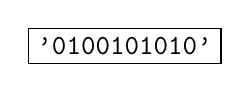
\begin{tikzpicture}
\def\uniteCodage{0.4cm}
\tikzset{codage/.style={anchor=south west,rectangle,minimum width=\uniteCodage},minimum height = \uniteCodage};
\node[codage,draw] at (0,0) {\texttt{'0100101010'}};
\end{tikzpicture}

\textit{{Codage de la rangée de briques}}
\end{center}
%\caption{Codage de la rangée de briques}
%\label{fig:exempleCodage}
%\end{subfigure}
%\caption{Illustration du codage choisi}
%\label{fig:codage}
%\end{figure}

Dans le détail, le \textit{i}\up{ième} élément (chiffre) de la chaîne de caractère indique si au niveau de la \textit{i}\up{ième} unité de longueur il y a oui ou non une jointure entre deux briques (\texttt{'1'} si il y a une jointure, \texttt{'0'} sinon). On n'inclut pas les deux extrémités - ce qui donne :

%\begin{figure}[h]
%\centering
\begin{tikzpicture}
\node[brique2,draw] at (0,0) {};
\node[brique3,draw] at ({2*\unite},0) {};
\node[brique2,draw] at ({5*\unite},0) {};
\node[brique2,draw] at ({7*\unite},0) {};
\node[brique2,draw] at ({9*\unite},0) {};

% valeurs
\def\uniteCodage{0.4cm}
\tikzset{valeur/.style={anchor=north}};
\node[valeur] (N1) at ({1*\unite},{-1*\uniteCodage}) {\texttt{'0}};
\node[valeur] (N2) at ({2*\unite},{-1*\uniteCodage}) {\texttt{1}};
\node[valeur] (N3) at ({3*\unite},{-1*\uniteCodage}) {\texttt{0}};
\node[valeur] (N4) at ({4*\unite},{-1*\uniteCodage}) {\texttt{0}};
\node[valeur] (N5) at ({5*\unite},{-1*\uniteCodage}) {\texttt{1}};
\node[valeur] (N6) at ({6*\unite},{-1*\uniteCodage}) {\texttt{0}};
\node[valeur] (N7) at ({7*\unite},{-1*\uniteCodage}) {\texttt{1}};
\node[valeur] (N8) at ({8*\unite},{-1*\uniteCodage}) {\texttt{0}};
\node[valeur] (N9) at ({9*\unite},{-1*\uniteCodage}) {\texttt{1}};
\node[valeur] (N10) at ({10*\unite},{-1*\uniteCodage}) {\texttt{0'}};

%relier
\draw[>=stealth,->] (N1.north) -- ({1*\unite},0);
\draw[>=stealth,->] (N2.north) -- ({2*\unite},0);
\draw[>=stealth,->] (N3.north) -- ({3*\unite},0);
\draw[>=stealth,->] (N4.north) -- ({4*\unite},0);
\draw[>=stealth,->] (N5.north) -- ({5*\unite},0);
\draw[>=stealth,->] (N6.north) -- ({6*\unite},0);
\draw[>=stealth,->] (N7.north) -- ({7*\unite},0);
\draw[>=stealth,->] (N8.north) -- ({8*\unite},0);
\draw[>=stealth,->] (N9.north) -- ({9*\unite},0);
\draw[>=stealth,->] (N10.north) -- ({10*\unite},0);

\end{tikzpicture}

%\end{figure}


\subparagraph{}\textit{Dessiner la rangée de briques correspondant à la chaîne de caractère suivante : \texttt{'0100100'}. De quelle taille est cette rangée ?}

%%\reponsebox{1.75cm}

%%\corrigebox{
\ifprof
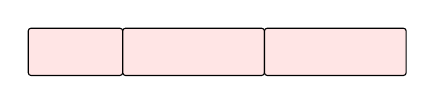
\begin{tikzpicture}
\def\unite{0.6cm}
\tikzset{brique/.style={anchor=south west,rectangle, rounded corners =1pt,minimum height = \unite,fill=red!10}};
\node[brique,minimum width={2*\unite},draw] at (0,0) {};
\node[brique,minimum width={3*\unite},draw] at ({2*\unite},0) {};
\node[brique,minimum width={3*\unite},draw] at ({5*\unite},0) {};
\end{tikzpicture}.
La rangée de briques est : 1 brique de taille 2, puis 2 de taille 3, soit une rangée de
taille \fbox{8}.%}
\else
\fi

%Maintenant, on suppose fixée à l'avance la longueur des murs que l'on souhaite compter. On appellera cette variable \texttt{tailleMax}.


\subparagraph{}\textit{\'Ecrire une fonction \texttt{imprimeRangee(rangee)} qui prend en argument une liste des deux chiffres 2 et 3 correspondant à une rangée de briques et qui renvoie la rangée de briques sous la forme codée (type \texttt{string}). Exemple : \texttt{imprimeRangee([2,3,2,2,2])} renvoie \texttt{'0100101010'}.}

%\reponsebox{4cm}

%\corrigebox{\pythonexternal{imprimeRangee.py}}


Deux rangées sont dites compatibles si elles peuvent être placées l'une sur l'autre, c'est-à-dire que les jointures ne sont pas au même endroit.

\subparagraph{}\textit{\'Ecrire une fonction}

\textit{ \texttt{sontCompatibles(r1,r2)} prenant en argument \texttt{r1} et \texttt{r2}, 2 rangées de briques sous la forme codée (type \texttt{string} - ex : \texttt{'011100'}), et qui renvoie \texttt{True} si les deux rangées données sont compatibles, \texttt{False} sinon.}

%\reponsebox{5cm}

%\corrigebox{\pythonexternal{sontCompatibles.py}}


%%%%%%%%%%%%%%%%%%%%%%%%%%%%%%%%%%%%%%%%%
%%%%%%%%%%% resolution %%%%%%%%%%%%%%%%%%
%%%%%%%%%%%%%%%%%%%%%%%%%%%%%%%%%%%%%%%%%

\subsection*{Résolution du problème}
\label{sec:resolution}



Pour dénombrer le nombre de façons différentes de construire un mur de longueur $l$ et de hauteur $h$, on adopte le principe de résolution suivant :
\begin{itemize}
\item \textbf{phase 1 :} déterminer toutes les combinaisons possibles des briques permettant de construire une rangée de longueur $l$. Par exemple, il n'y a que deux façons possibles pour les rangées de longueur 5 : une brique de longueur 2, puis une brique de longueur 3 ; et l'inverse. Les codages correspondants sont : \texttt{'0100'} et \texttt{'0010'}. Soit $R$ l'ensemble de ces codages de rangées de briques;
\item \textbf{phase 2 :} pour chaque rangée $r$ de $R$, déterminer le nombre de murs de hauteurs $h$ dont la première rangée de briques (celle tout en bas) est $r$. Cette valeur est notée \texttt{compteRangee(R, r, h)};
\item \textbf{phase 3 :} calculer $\sum \limits_{r \in R} \mathtt{compteRangee(R,r,h)}$ pour toutes les rangées possibles de longueur $l$. C'est le résultat final attendu.
\end{itemize}


%Dans la suite, l'objectif est de comprendre l'algorithme récursif de la phase 2, puis de l'améliorer.


\subsection*{\'Etude de la phase 1}
\label{ssec:phase1}

Dans un premier temps, on aimerait connaître le nombre de combinaisons possibles distinctes afin de remplir la rangée de briques avec des briques élémentaires de dimensions 2 et 3.

\subparagraph{}\textit{Proposer une fonction récursive \texttt{combinaisons(l)} prenant en argument la longueur du mur $l$ et renvoyant le nombre de solutions possibles distinctes afin de remplir une rangée. Vous pourrez construire votre algorithme en vous appuyant sur un schéma (arbre) ayant pour sommet $l=11$.}
%\reponsebox{9cm}

%\corrigebox{\pythonexternal{combinaisons.py}}

\subparagraph{}\textit{Préciser la complexité de votre fonction.}
%\reponsebox{4 cm}
%\corrigebox{On a : $C(n)=C(n-2)+C(n-3)$, alors on obtient une complexité en $C(n)=O\left(\lambda^n \times 2^{n}\right)$ soit \fbox{une complexité exponentielle}.}

Pour la phase 1, on suppose écrite une fonction \texttt{remplissage(l)} qui renvoie la liste de toutes les rangées possibles de longueur $l$. Par exemple, \texttt{remplissage(5)} renvoie les deux rangées : \texttt{'0100'} et \texttt{'0010'}.








%Le code de la fonction toutes les lignes vous est donné blabla (à décider..)

\subparagraph{}\textit{Sans écrire aucun code, quelle serait la structure du code de la fonction \texttt{remplissage} ?}

%\reponsebox{6cm}

%\corrigebox{
\ifprof
\else
Il est nécessaire de créer une fonction récursive qui ajoute dans la branche de gauche une brique de 2 (concaténation de la chaîne de caractère en cours avec \texttt{'10'}), puis dans la branche de droite une brique de trois (concaténation de la chaîne de caractère en cours avec \texttt{'100'}). Il faut gérer la longueur du mur en cours (\texttt{w} dans le code ci-dessous) - ceci constituera notre cas de base dès lors que le mur en cours fera la longueur souhaitée. Enfin, il faut remplir une liste de toutes les combinaisons. J'ai utilisé une variable globale (très utile ici), en s'appuyant sur la génération pour une brique initialement de 2 puis une de 3. Le code à titre informatif:
%\pythonexternal{remplissage.py}
 %}
\fi

\subsection*{\'Etude de la phase 2}
\label{ssec:phase2}

Pour dénombrer les murs (phase 2 de la résolution), on utilise une fonction récursive \texttt{compteRangee(R, r, h)}
qui détermine le nombre de murs dont la première rangée de briques est $r$ et dont la hauteur est $h$.
L'objet de cette sous-section est de comprendre cet algorithme et son implémentation, qui sont donnés dans le fichier macon.py%en page~\pageref{LastPage}.

\subparagraph{}\textit{Pourquoi la quantité \texttt{compteRangee(R, r, 1)} vaut-elle 1 pour tout $r$ ?}
%\reponsebox{3cm}

%\corrigebox{Parce qu'il n'y a qu'une seule façon de faire un mur de hauteur 1 avec une rangée donnée !}


\subparagraph{}\textit{On suppose $l = 5$. Développer sur votre copie les différentes étapes de calcul (avec les
appels récursifs) de l'appel \texttt{compteRangee(combinaisonsCinq,combinaisonsCinq[0],2)}, \texttt{combinaisonsCinq} étant la liste comportant les deux chaînes de caractères, \texttt{'0100'} et \texttt{'0010'}, codant les rangées.
}
%\reponsebox{8cm}

%\corrigebox{On va donc dérouler les appels récursifs (arbre) :
\ifprof
\begin{itemize}
\item appel à \texttt{compteRangee(combinaisonsCinq,'0100',2)}
\item initialement, \texttt{somme} vaut 0 ; nbCombi vaut 2 ; i vaut 0
\item i<2 ici 0<2 vrai
\item SontCompatibles('0100','0100') False ; i=i+1=1
\item i<2 ici 1<2 vrai
\item SontCompatibles('0010','0100') True
\begin{itemize}
\item appel à \texttt{compteRangee(combinaisonsCinq,'0010',1)}
\item h=1 ; la fonction renvoie 1 ; somme=somme+1=1
\item i=2 ; boucle while interrompue
\end{itemize}
\item à la fin \texttt{somme} vaut 1, et on renvoie 1.
\end{itemize}
%}
\else
\fi
%\subparagraph{}\textit{Démonter en exhibant un invariant de boucle que la fonction proposée permet de renvoyer le résultat attendu. Préciser le variant. }
%
%%\reponsebox{10cm}
%
%%\corrigebox{}




\subsection{\'Etude de la phase 3}
Afin de réaliser l'objectif, la fonction \texttt{compteTout(toutesLesCombinaisonsLigne,hauteur)} sera écrite. 


\subparagraph{}\textit{\'Ecrire la fonction \texttt{compteTout(toutesLesCombinaisonsLigne,hauteur)} prenant en argument une liste de chaînes de caractères et la hauteur du mur souhaitée, et renvoyant un entier nombre de combinaisons possibles afin de construire le mur d'une manière correcte.}
%\reponsebox{8cm}
%\corrigebox{\pythonexternal{compteTout.py}}


Dans cette sous-section, nous chercherons les limites de notre algorithme naïf proposé dans la sous-section précédente, et nous chercherons donc à l'améliorer.

\subparagraph{}\textit{En s'appuyant sur le calcul des murs de longueur 9 et de hauteur 3, donner le principal défaut de l'algorithme naïf proposé précédemment.}

%\reponsebox{4cm}

%\corrigebox{Pour le calcul des murs de longueur 9 et de hauteur 3, une bête réflexion au début de chaque appel récursif nous montre que l'on appelle deux fois \texttt{compteRangee(toutesLesCombinaisons,'00100100',2)}. Ce phénomène se répétant très souvent, il rend très lent notre algorithme.}


\subparagraph{}\textit{Proposer alors une amélioration de l'algorithme.}

%\reponsebox{4cm}

%\corrigebox{
\ifprof
Si on reprend l'exemple précédent, on peut donc effectuer
ce calcul une fois, puis stocker ce nombre dans une table. Cela devient très fortement intéressant à partir du moment où l'on demande par exemple le calcul des murs de longueur 30 et de hauteur 10.
\else
\fi
%
%%
%%%\newpage
%%\begin{center}
%%\begin{Huge}
%%\fbox{Annexe}
%%\end{Huge}
%%\end{center}
%\subsection*{Annexe}
%\begin{python}
%def compteRangee(toutesLesCombinaisonsLigne,r,hauteur):
%    if hauteur==1:
%        return(1)
%    else:
%        nbCombi=len(toutesLesCombinaisonsLigne)
%        somme=0
%        i=0
%        while i<nbCombi:
%            if sontCompatibles(r,toutesLesCombinaisonsLigne[i]):
%                somme+=compteRangee(toutesLesCombinaisonsLigne,toutesLesCombinaisonsLigne[i],hauteur-1)
%            i+=1
%        return(somme)
%\end{python}



\ifprof
\else
\end{multicols}
\fi
%\begin{thebibliography}{2}
%\bibitem{1}{Patrick Beynet, \textit{Supports de cours de TSI 2}, Lycée Rouvière, Toulon.}
%\bibitem{2}{<< Mandel zool 08 satellite antenna >>. Sous licence CC BY-SA via Wikimedia Commons - 
%\url{https://fr.wikipedia.org/wiki/Ensemble_de_Mandelbrot#/media/File:Mandel_zoom_08_satellite_antenna.jpg}}
%\bibitem{3}{\url{http://www.obside.fr/fractales/pages/Recursif/}}
%\end{thebibliography}
\end{document}

